\section{Introduction}
\label{sec:intro}

Enabling high-performance execution of deep neural networks (DNNs) on GPUs is critical for modern ML applications. 
Today's DNN frameworks generally specify DNN computation using tensor programs, which are directed acyclic graphs whose nodes and edges represent tensor algebra operators (e.g., matrix multiplication) and tensors (i.e., $n$-dimensional arrays) shared between operators. 

To optimize an input tensor program, existing frameworks (e.g., PyTorch~\cite{pytorch} and TensorFlow~\cite{Tensorflow}) use manually designed rules to map the tensor program to expert-written GPU kernels.
These approaches generally require extensive engineering efforts to design and implement optimization rules, and they may miss certain optimization opportunities.
To address these challenges, recent work has introduced {\em automated} approaches that optimize tensor programs by searching over a comprehensive space of program transformations and applying them based on their performance on target GPUs.
These approaches generally fall into two categories.

The first category of work, including Halide~\cite{halide}, TVM~\cite{tvm}, and Ansor~\cite{ansor}, is motivated by the idea of algorithm and schedule separation\footnote{In the schedule optimization literature, an algorithm describes what to compute in a kernel and a schedule specifies how to compute the kernel.} introduced in Halide and optimizes the {\em schedule} of a tensor program while fixing the algorithm.
%
For a given algorithm, these optimizers automatically generate performant kernels by searching for possible strategies to execute the kernel on the target hardware.
However, due to the linear algebra nature of DNNs, a tensor program can be represented by a wide spectrum of mathematically equivalent algorithms. Existing schedule-based optimizers only consider kernels whose algorithms are manually specified by users, resulting in missed optimization opportunities.
%tensor program, they automatically generate high-performance kernels by searching over potential schedules, each of which represents an architecture-dependent strategy for executing the program on the target hardware. 

The second category of work, including TASO, Grappler, Tensat, and PET, considers {\em algebraic transformations}, which exploit mathematical equivalence among different algorithms for a tensor program~\cite{TASO, tensorflow_grappler, yang2021equality, wang2021pet}. 
%
Examples of algebraic transformations include (1) converting one linear algebra operator into another, such as transforming a convolution to a matrix multiplication; (2) fusing multiple operators to reduce memory access and kernel overhead; and (3) reorganizing operators based on commutativity, associativity, and distributivity.
%transforming the graph structure of tensor programs.
%reordering operators to improve computational efficiency by linear algebra properties of operators, (2) replacing less efficient operators with more optimized ones, and (3) transforming the graph structure of a tensor program.
%
These optimizers perform algebraic transformations at the algorithm level and require programmers to manually specify the set of available operators and their implementations.
%
They are thus limited by the performance of the provided kernels.

%These algorithm optimizers perform {\em algebraic transformations} to explore the search space of mathematically equivalent algorithms for an input tensor program to discover a highly efficient algorithm.

%\ZJ{Both existing approaches require manually defined kernels and are limited to the provided kernels.}

All existing automated optimization approaches, from both categories, still require programmers to manually specify a set of kernels (each defined by a tensor function), and then explore the search space of algebraic {\em or} schedule transformations.
%Existing automated tensor program optimizers only explore the search space of algebraic {\em or} schedule transformations, while relying on heuristics or manually designed rules to apply transformations in the other category.
%
%However, many advanced performance optimizations use highly sophisticated algorithms for kernels and require combining algebraic and schedule transformations at the kernel, thread block, and thread levels of GPU compute hierarchy, which are beyond the search space of existing automated methods and still require manual implementation.
However, some advanced performance optimizations require coordinated transformations across the kernel, thread block, and thread levels of the GPU compute hierarchy, and involve introducing completely new kernel computations (e.g., a custom kernel that decomposes standard kernels and fuses only certain computations).
Such optimizations are not included in the search space of existing automated methods and must still be implemented manually.

One such example is FlashAttention~\cite{dao2023flash} (see \S\ref{subsec:benchmark_results} for details), which optimizes attention~\cite{transformers} on GPUs by reordering operators at the algorithm level (algebraic transformations), reorganizing the computation across GPU kernels (yielding new custom kernels), and adapting the parallelization strategy of each kernel to the GPU architecture (schedule transformations).
%
The transformations required for this example cannot be automatically discovered by existing frameworks and must therefore be implemented manually.
%
%These optimizations require collectively applying algebraic and schedule transformations at multiple levels in the GPU compute hierarchy, which cannot be automatically discovered by existing frameworks and require extensive engineering effort to implement them manually.
%
%These optimizations require collectively applying transformation at multiple levels in the GPU compute hierarchy, which cannot be automatically discovered by existing frameworks and require extensive engineering effort to implement them manually.
%Due to the necessity of combining algebraic and schedule transformations at multiple levels, these optimizations cannot be automatically discovered by existing frameworks and require extensive engineering effort to implement them manually.
%
%Supporting FlashAttention in existing tensor program optimizers such as Triton or TVM requires users to manually specify (1) how to reorganize and decompose the computation into multiple kernels and (2) the order of computation in each kernel. 
An implementation of FlashAttention in Triton~\cite{tillet2019triton}, a widely used tensor program optimizer, contains more than 700 lines of code~\cite{triton-flashattention}.

%\ZJ{Old version.} Existing automated approaches to optimizing tensor programs {\em separately} apply algebraic and schedule transformations. 
%For example, most DNN frameworks first apply graph-level optimizations for algebraic transformations and then perform schedule transformations to generate a kernel for each operator.
%Although widely used, this approach cannot automatically discover complex optimizations that require combining algebraic and schedule transformations.
%One such example is FlashAttention~\cite{dao2023flash} (see \Cref{sec:case} for details), which maximizes GPU shared memory reuse by simultaneously reorganizing tensor operators (i.e., algebraic transformations) and how these operators are executed (i.e., schedule transformations).
%Due to the necessity of combining algebraic and schedule transformations at multiple levels, these optimizations cannot be automatically discovered by existing frameworks and require extensive engineering effort to implement them manually.

%\ZJ{Note sure if we need this paragraph: This paper aims to answer the following research question: how can we automatically discover and verify tensor program optimizations that include and outperform those manually designed by experts?}

We present \sys, the first {\em multi-level superoptimizer} for tensor programs.
%
\sys automatically discovers and verifies sophisticated optimizations of tensor programs that require joint optimization of algebraic transformations, schedule transformations, and the discovery of new custom kernels. 
%

A key idea in \sys is \graphs, a {\em hierarchical graph representation} that specifies tensor programs across multiple levels of the GPU compute hierarchy.
%
By uniformly treating the kernel, thread block, and thread levels, \graphs can capture both algebraic and schedule transformations across these levels.
Moreover, optimizing a \graph can introduce new custom kernels, which go beyond both algebraic and schedule transformations.
%
%\graph unifies the representation of algebraic and schedule transformations in a hierarchical graph structure and interleaves these two types of optimizations at the kernel, thread block, and thread levels, making \graph capable of representing various joint optimizations of algebraic and schedule transformations.
%
For example, \sys automatically discovers the \graphs representing FlashAttention~\cite{dao2023flash} and its inference variant FlashDecoding~\cite{tri2023flashdecoding} as well as other \graphs that outperform these manually designed kernels by up to 2.2$\times$ for certain use cases.
%using the \graph representation, \sys automatically discovers FlashAttention as well as other \graphs that outperform FlashAttention.
Most of these optimizations discovered by \sys are outside the search space of existing methods.
%\sys includes two key components:

\begin{figure}
    \centering
    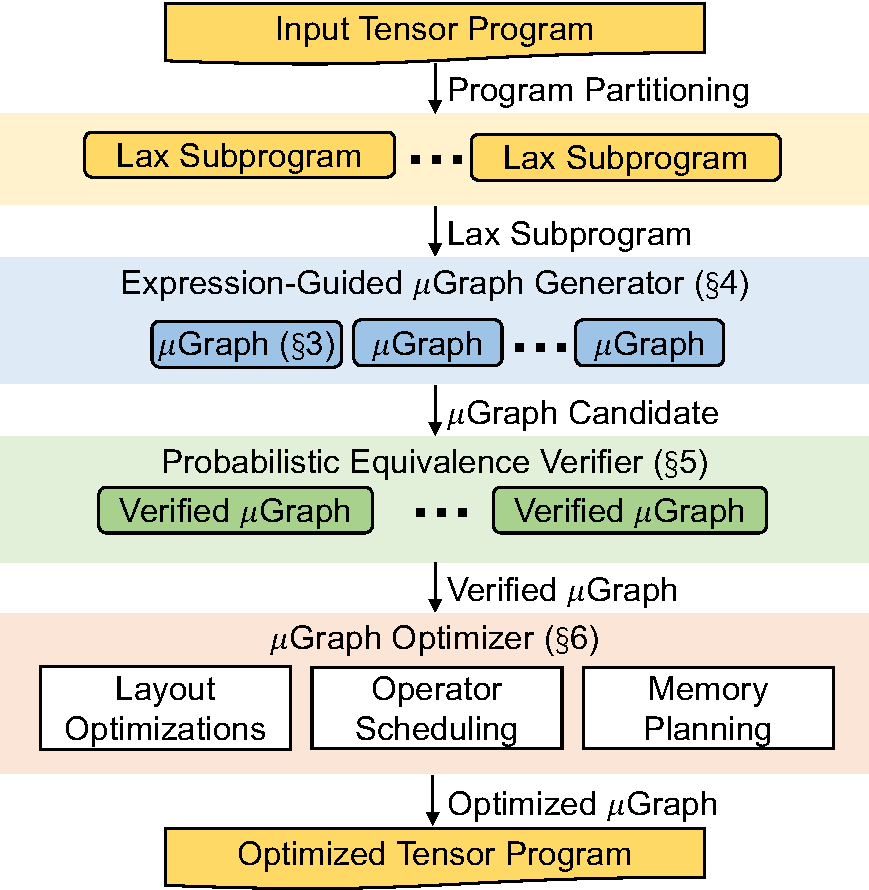
\includegraphics[scale=0.48]{figs/overview3-crop.pdf}
    \vspace{\captionvspace}
    \caption{An overview of \sys.}
    \vspace{-1em}
    \label{fig:overview}
\end{figure}

\Cref{fig:overview} shows an overview of \sys.
\sys first splits an input tensor program into subprograms that fall into the restricted \lax fragment.
The \lax fragment, formally defined in \S\ref{sec:verify}, includes multi-linear operators such as matrix multiplication and convolution, division (useful for normalizations), and limited exponentiation (useful for activations).
%a certain class of tensor programs termed \lax programs, which includes 
%\Cref{fig:overview} shows an overview of \sys, which takes a tensor program as input and produces an executable for the program. \sys first splits the input program into a certain class of tensor programs termed \lax programs, which includes 
%\footnote{\lax stands for \underline{l}inear, division, and \underline{a}n e\underline{x}ponential.} (defined below).
%\lax programs capture the compute-intensive components of a tensor program, and this partitioning reduces the exploration space of each subprogram while preserving most optimization opportunities.
%\oded{I'm not sure about the previous sentence}
%
Partitioning a tensor program into \lax subprograms reduces the optimization search space while preserving most optimization opportunities; it also enables \sys's probabilistic equivalence verifier.
%
%For example, attention~\cite{transformers} is itself a \lax program, and \sys's partitioning strategy preserves optimizations for attention.

\paragraph{Expression-guided \graph generator.}
For each \lax subprogram, \sys's {\em expression-guided generator} exhaustively searches for possible \graphs equivalent to it.
A key challenge \sys must address is its significantly larger search space compared to prior superoptimization techniques.
%
%For example, TASO~\cite{TASO} and PET~\cite{wang2021pet} search only for tensor programs at the kernel level, using a fixed set of pre-defined kernels, while \sys simultaneously considers superoptimization across the kernel, thread block, and thread levels.
For example, TASO~\cite{TASO} and PET~\cite{wang2021pet} search only for tensor programs at the kernel level, using a fixed set of pre-defined kernels, while \sys considers superoptimization across the kernel, thread block, and thread levels.
%
%To efficiently navigate this significantly larger and more complex search space, \sys introduces a novel pruning technique based on {\em abstract expressions}.
To efficiently navigate this significantly larger search space, \sys introduces a novel pruning technique based on {\em abstract expressions}, which greatly reduces the number of \graphs \sys must consider while providing a certain theoretical guarantee on the optimality of the discovered \graphs.
\sys further reduces the search space by focusing the search on the kernel and block levels and using a rule-based approach for the thread level. 

%based on the observation that the most important optimization opportunities lie at the kernel and block level, \sys applies the pruning-assisted enumeration to those levels, and uses a more standard rule-based approach for optimizing the thread level, while maintaining the uniform \graph representation across all levels.

%Abstract expressions allow \sys to ignore many \graphs that are not even abstractly equivalent to the desired \lax program. 
%\oded{what do you think about this sentence?}
%\MW{I think we are using `abstractly' before giving any intuition on it, so `not even abstractly equivalent to' does not explain a lot.}
%, which is a signature of each tensor in a \graph that represents how the tensor is computed from the program's inputs while ignoring differences between elements from the same input tensor. \MW{Need to update to align with updated sec 5.3}
%
%\sys leverages the sub-expression relationships between tensors to guide \graph generation and filters out \graphs that cannot yield the final output of the input \lax program.
%
%This approach greatly reduces the number of \graphs \sys must consider while providing a theoretical guarantee on the optimality of the discovered \graphs (\S\ref{subsec:abstract_expression}).
%
%All \graphs with the same abstract expression as the input \lax program are considered as candidate \graphs.

\paragraph{Probabilistic equivalence verifier.}
For a \graph discovered by \sys, verifying its functional equivalence with the input program introduces another challenge, since the input and output tensors of a program include up to many millions of elements.
%Verifying functional equivalence of two \graphs introduces another challenge. 
A key idea behind \sys is {\em probabilistic equivalence verification}, which performs random tests over finite fields to check equivalence between \graphs.
%
%While random tests can hardly provide any correctness guarantees for general programs, \sys introduces a set of rigorous theoretical results to show that for a certain class of tensor programs termed \lax programs, random tests over finite fields offer strong correctness guarantees.
While random tests typically provide limited correctness guarantees for general programs, \sys leverages a novel theoretical result showing that the restrictions imposed by the \lax fragment ensure that, for \lax programs, random tests over finite fields offer strong correctness guarantees.
%We essentially show that an algorithm for polynomial identity testing (PIT)~\cite{schwartz1980fast, zippel1979probabilistic} can be generalized to \lax programs, yielding a randomized algorithm that can be made arbitrarily precise, that is, the probability of non-equivalent \graphs to pass the test can be made arbitrarily low.
Specifically, we show that a polynomial identity testing (PIT) algorithm~\cite{schwartz1980fast, zippel1979probabilistic} can be generalized to \lax programs, yielding a randomized algorithm for \lax program equivalence that can be made arbitrarily precise.
\sys uses this randomized algorithm to (probabilistically) ensure that each optimized program is equivalent to the input program.
%
%\oded{I think the following can be significantly shortened or removed:}\MW{I agree we can just remove them.}
%
%First, functionally equivalent \graphs always pass random tests, and \sys's verifier always verifies their equivalence.
%Second, for non-equivalent \graphs, the verifier detects that they are not equivalent with a certain probability.
%\sys's verifier can repeat the probabilistic equivalence verification process multiple times to reduce the error rate (i.e., two non-equivalent \graphs pass all random tests) to an arbitrarily low threshold.
%This approach allows \sys to trade-off accuracy and efficiency of the verifier and can achieve arbitrarily high accuracy by repeating the verification steps.
%'s approach to automatically verifying a \graph is to use multiple {\em random tests} executed in finite fields of integers.
%\sys uses a set of rigorous theoretical foundations to show that random testing can provide a certain degree of correctness guarantee and repeated random tests can significantly boost this correctness guarantee and reduce the error probability to an arbitrarily small threshold. 

\paragraph{\graph optimizer.} For each verified \graph, \sys's {\em \graph optimizer} maximizes its runtime performance by further considering potential tensor layouts, scheduling operator execution orders, and planning memory allocation at all of the kernel, thread block, and thread levels.
%
Finally, \sys returns an optimized tensor program based on the best discovered \graph for each individual \lax subprogram.


\paragraph{Evaluation results.}
We evaluate \sys on a variety of commonly used DNN benchmarks on NVIDIA A100 and H100 GPUs.
%12 benchmarks commonly used in today's DNNs, including different variants of attention~\cite{ainslie2023gqa, transformers, shazeer2019mqa}, low-rank adaptation~\cite{hu2021lora}, and multi-layer perceptron~\cite{houlsby2019parameter}.
%\oded{say something like: that represent state-of-the-art..., otherwise 12 sounds kind of low}
Even for DNN benchmarks that are widely used and heavily optimized by existing systems, such as the group-query attention used in LLMs~\cite{grattafiori2024llama3herdmodels}, \sys still outperforms current approaches by up to 3.3$\times$ by exploiting subtle custom kernels and optimizations missing in existing systems.
%\MW{TODO:update the number}
%
%Most optimizations discovered by \sys use subtle custom kernels and combine algebraic and schedule transformations at multiple levels of the GPU hierarchy, which are missing in existing systems.
%\oded{also new custom kernels?}
%
\if 0
\ZJ{Needs update.}
In summary, this paper makes the following contributions:
(1) the first superoptimizer for tensor programs that simulatiosly operates at the kernel, thread block, and thread levels;
(2) the \graph representation, a uniform representation of computations across multiple levels that unifies algebraic and schedule transformations and supports discovery of new custom kernels;
(3) the expression-guided generator for exploring the large and complex search space of \graphs by leveraging abstract expressions to prune the search space;
and (4) \oded{what's (4)? I guess it's the probabilistic verification?}
\fi 

\if 0
For the rest of this paper, \S\ref{sec:hcg} and \S\ref{sec:case} introduce the \graph representation and use a case study to demonstrate its advantages, \S\ref{sec:overview} presents an overview of the \sys framework, \S\ref{sec:search} describes the expression-guided generator, \S\ref{sec:verify} introduces the probabilistic equivalence verifier, \S\ref{sec:eval} evaluates \sys by comparing its performance with existing systems, \S\ref{sec:related} relates \sys to prior work, and \S\ref{sec:conclusion} concludes.
\fi